%!TEX root = ../Main.tex
\begin{wrapfigure}[7]{r}{.3\textwidth}
	\vspace{-2.3em}
	\centering
	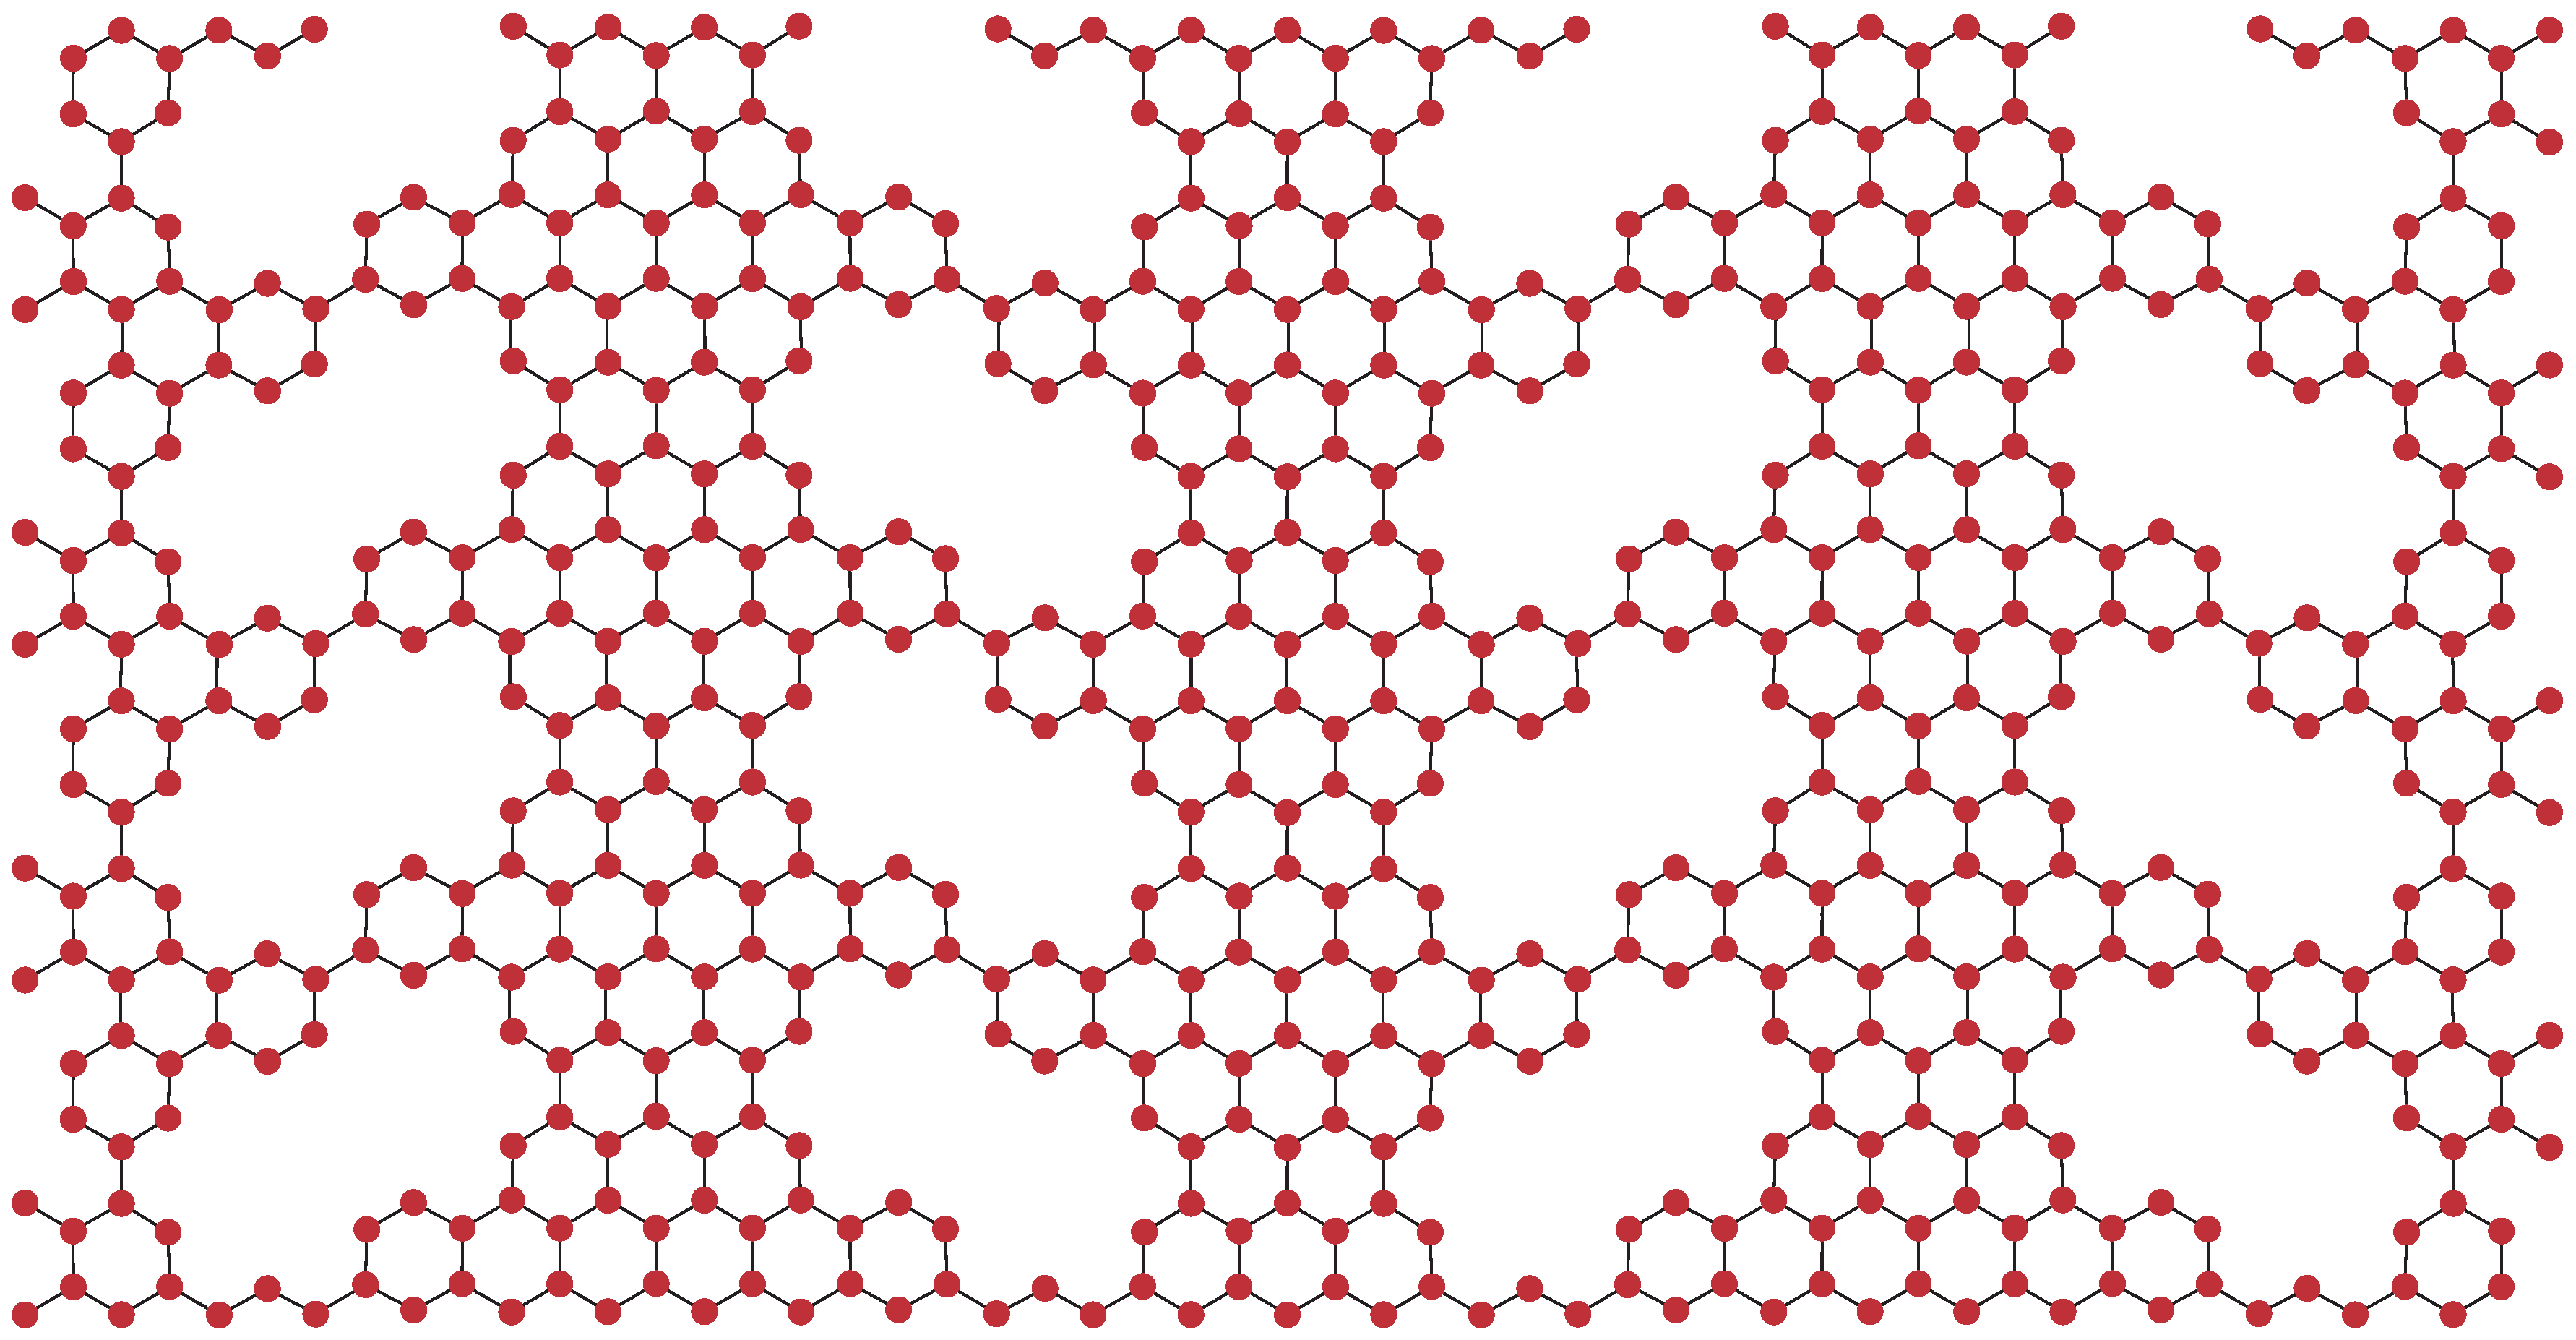
\includegraphics[width=.4\textwidth]{Figures/NPGintroGraphic.eps}
    \caption{Drawing of a nanoporous graphene device.}\label{introGraphic}
\end{wrapfigure}
In recent years so called nano-porous graphene devices (NPGs) has been proposed for various applications. [Insert litt.] These devices are made up of single layered graphene with periodic holes (hence the porous). The remaining graphene constitutes ribbons and bridges in the structures. \cref{introGraphic} shows how one such structure can look like.
Because of graphenes electrical properties [Insert litt], one should be able to finely control the electron currents in the devices and thus create nanometer circuits for use as e.g. chemical detectors. As a result of its novelty, the fabrication of such devices are limited. Before fabrication one must show promising effects through theoretical simulations.\newline
This project focuses on the development of numerical routines in Python by employing NumPy. We implementing the tight-binding approximation on NPGs. The transport can then be simulated using Green's functions as well as clever recursion algorithms. From here we obtain transmission and band structures for simulated devices.\newline
Generally speaking the community uses DFT-based simulations through tools like those from the SIESTA project (TBtrans). Results are then analysed using SISL\cite{zerothi_sisl}. The DFT results can then be extrapolated to larger scales\cite{calogero_electron_2019}. However DFT programs might seem as a blackbox. To get a better understanding of electron transport, we avoid DFT and rely solely on tight-binding simulations. We then confirm the validity of the developed products by comparing result to those from SIESTA.\newline
The main scope is the development of the tight-binding scripts, comparing results with those of DFT calculations and discuss whether a clean tight-binding approach can sufficiently be used for the relatively simple NPGs.\newline
To summarise:
\begin{enumerate}
	\item Apply quantum mechanics for electron transport in NPGs.
	\item Use numerical methods (recursion algorithms, linear algebra) with NumPy to implement tight-binding.
	\item Calculate band structures and transmission plots for various devices.
	\item Gather single-particle Green’s functions and LDOS of said devices.
	\item Compare the obtained results and discuss whether or not they sufficiently ressemble DFT based simulations.
\end{enumerate}
The report is organised on the following way:
\begin{enumerate}
	\item \cref{theorysec,hamilsec,greensec,transec} deals with the development of our methodology. By introduction of basic theoretical concepts, followed by how these concepts are implemented practically through programming.
	\item \cref{testsec} deals with the generated result on various NPGs and the comparison with DFT calculations with similar systems.
\end{enumerate}
The code repository (which also includes the \latex files for this report) can be found on Github: \faGithub \ \url{https://github.com/rwiuff/QuantumTransport}
